\documentclass[12pt,a4paper]{article}
\usepackage[utf8]{inputenc}
\usepackage[T2A]{fontenc}
\usepackage[russian]{babel}
\usepackage{graphicx}
\usepackage{booktabs}
\usepackage{longtable}
\usepackage{array}
\usepackage{geometry}
\usepackage{amsmath}
\usepackage{amsfonts}
\usepackage{float}
\usepackage{paracol}
\usepackage{src/title}
\usepackage{hyperref}
\usepackage{listings}
\usepackage{xcolor}

\geometry{top=2cm, left=2cm, right=2cm, bottom=2cm}

\DeclareMathOperator{\rank}{rank}

\title{Лабораторная работа №6. Сингулярное разложение матриц и его применение}

\author{%
    Аннуфриев Андрей Сергеевич (465029)\\
    Бахуров Николай Алексеевич (504862)\\
    Раджапов Фёдор Сергеевич (502544)%
}

\supervisor{Зарина Ольга Андреевна}

\date{01.11.2026}

\hypersetup{
    pdftitle={PLA Lab 6 SVD image compression and LSA},
    pdfauthor={Anufriev Andrey Sergeevich, Bakhurov Nikolai Alekseevich, Rajapov Fedor Sergeevich},
    pdfsubject={Singular Value Decomposition, image compression, LSA},
    linkcolor=blue,
    filecolor=magenta,
    urlcolor=cyan
}

\definecolor{codegreen}{rgb}{0,0.6,0}
\definecolor{codegray}{rgb}{0.5,0.5,0.5}
\definecolor{codepurple}{rgb}{0.58,0,0.82}
\definecolor{backcolour}{rgb}{0.95,0.95,0.92}

\lstdefinestyle{codestyle}{
    backgroundcolor=\color{backcolour},
    commentstyle=\color{codegreen},
    keywordstyle=\color{magenta},
    numberstyle=\tiny\color{codegray},
    stringstyle=\color{codepurple},
    basicstyle=\ttfamily\footnotesize,
    breakatwhitespace=false,
    breaklines=true,
    captionpos=b,
    keepspaces=true,
    numbers=left,
    numbersep=5pt,
    showspaces=false,
    showstringspaces=false,
    showtabs=false,
    tabsize=2
}
\lstset{style=codestyle}

\abstract{
    В работе исследуется сингулярное разложение матриц (SVD) на двух прикладных примерах:
    сжатие grayscale-изображения и латентный семантический анализ текстовой коллекции (LSA).
    Для изображения построены усечённые SVD-реконструкции при девяти значениях параметра
    $k$, оценены степень сжатия и ошибка реконструкции. Для текстового состава составлена
    терм-документная матрица, выполнено её SVD, выделены две латентные темы по топ-5 словам
    из первых двух сингулярных векторов и подобраны соответствующие документы. Построены
    две диаграммы «облако слов». Приведены ответы на восемь контрольных вопросов.
}

\keywords{сингулярное разложение; сжатие изображений; латентный семантический анализ;
терм-документная матрица; сингулярные числа}

\begin{document}
\sloppy
\maketitle
\tableofcontents
\newpage

\section{Цели и задачи}
Цель работы — ознакомиться с двумя применениями сингулярного разложения матриц и получить
практические навыки вычисления SVD на Python.

\textbf{Задание 1 (сжатие изображений).} Выбрать изображение, перевести его в оттенки
серого и рассмотреть как матрицу $A$ размера $m\times n$. Выполнить полное SVD-разложение
$A = U\Sigma V^\top$. Построить усечённое SVD, оставив только $k$ первых (наибольших)
сингулярных чисел и соответствующие векторы, и вывести восстановленное изображение — не
менее чем при девяти различных значениях $k$. Сделать выводы о влиянии параметра $k$ на
качество изображения и степень сжатия (доля исходной информации, которую необходимо
хранить в памяти), а также оценить степень сжатия численно при каждом $k$.

\textbf{Задание 2 (LSA).} Выбрать текстовый файл — коллекцию документов. Удалить знаки
препинания и разбить текст на слова, выполнить лемматизацию, исключить шумовые слова.
Составить словарь и терм-документную матрицу, описывающую частоты терминов в документах.
Выполнить SVD этой матрицы. Проанализировать первые два сингулярных числа и соответствующие
левые и правые сингулярные векторы: по топ-5 слов с наибольшим отклонением в соответствующих
векторах восстановить две основные темы и определить документы, которым эти темы
соответствуют в наибольшей степени. Построить две диаграммы «облако слов».

\section{Теоретические сведения}

\subsection{Сингулярное разложение матриц}
Любая вещественная матрица $A$ размера $m\times n$ разлагается как
\[
    A = U\Sigma V^\top,
\]
где $U$ ($m\times m$) и $V$ ($n\times n$) — ортогональные матрицы, столбцы которых —
левые и правые сингулярные векторы, а $\Sigma$ ($m\times n$) — диагональная матрица с
неотрицательными сингулярными числами $\sigma_1\ge\sigma_2\ge\dots\ge0$ на диагонали.

Геометрический смысл: отображение $x\mapsto Ax$ есть композиция поворота/отражения
($V^\top$), масштабирования по осям на $\sigma_i$ ($\Sigma$) и поворота/отражения ($U$).
Сингулярные числа показывают, насколько сильно отображение растягивает пространство
вдоль соответствующих собственных направлений.

Связь с собственными числами: столбцы $U$ — собственные векторы $AA^\top$, столбцы $V$ —
собственные векторы $A^\top A$, а $\sigma_i^2$ — собственные числа обеих матриц
($AA^\top$ и $A^\top A$ имеют одинаковые ненулевые собственные числа).

\subsection{Образ, ядро, ранг и псевдообращение}
\begin{itemize}
    \item $\rank(A)$ равен количеству ненулевых сингулярных чисел.
    \item $\operatorname{Im}(A)$ натянуто на левые сингулярные векторы, соответствующие
    ненулевым $\sigma_i$; $\operatorname{Ker}(A)$ — на правые сингулярные векторы
    с $\sigma_i=0$.
    \item Псевдообращение Мура — Пенроуза через SVD:
    \[
        A^+ = V\Sigma^+U^\top,\qquad
        (\Sigma^+)_{ii} = \begin{cases}1/\sigma_i,&\sigma_i>0,\\0,&\sigma_i=0.\end{cases}
    \]
    Свойства: $AA^+A=A$, $A^+AA^+=A^+$, $(AA^+)^\top=AA^+$, $(A^+A)^\top=A^+A$.
\end{itemize}

\subsection{Усечённое SVD и сжатие данных}
Усечённое SVD ранга $k$:
\[
    A_k = \sum_{i=1}^{k}\sigma_i\,u_i v_i^\top = U_k\Sigma_k V_k^\top,
\]
где $U_k$ ($m\times k$), $\Sigma_k$ ($k\times k$), $V_k^\top$ ($k\times n$).
По Эккарту — Янгу, $A_k$ — наилучшее приближение матрицы $A$ ранга не выше $k$ в норме
Фробениуса и спектральной норме.

При Approximation $A\approx A_k$ вместо всей матрицы $mn$ чисел достаточно хранить
$k(m+n+1)$ чисел (элементы $U_k$, $\Sigma_k$, $V_k^\top$). Степень сжатия (доля
исходных данных):
\[
    \gamma(k) = \frac{k(m+n+1)}{mn}.
\]
Если $\gamma(k)>1$, усечённое SVD занимает больше памяти, чем исходная матрица — такая
$k$ не даёт реального сжатия. Предел применимости: $k < mn/(m+n+1)$.

\subsection{Латентный семантический анализ (LSA)}
Пусть $A$ — терм-документная матрица размера (размер словаря)$\times$(число документов),
элемент $A_{tj}$ — частота термина $t$ в документе $j$. При SVD $A=U\Sigma V^\top$:
\begin{itemize}
    \item столбцы левой матрицы $U$ — ортонормированные базисные векторы в
    \emph{термин-пространстве} (латентные темы, выраженные через слова);
    \item столбцы правой матрицы $V$ (строки $V^\top$) — координаты документов в
    \emph{документ-пространстве} (какой документ относится к какой теме);
    \item сингулярные числа $\sigma_i$ показывают значимость (вес) соответствующих
    латентных тем: чем больше $\sigma_i$, тем сильнее тема выражена в коллекции.
\end{itemize}
Первые два сингулярных числа задают две доминирующие темы. По модулю компонент левых
сингулярных векторов $u_1,u_2$ выбираются топ-5 слов темы; по модулю компонент правых
векторов $v_1,v_2$ — наиболее соответствующие документы.

\section{Исходные данные}

\subsection{Изображение для Задания 1}
Исходное grayscale-изображение размером $1308\times 736$ пикселей (сгенерировано
синтетически в соответствии с допущением WORKLOG.md) рассмотрено как матрица
$A$ размера $1308\times 736$ пикселей. Полное SVD-разложение
$A=U\Sigma V^\top$ выполнено через \texttt{numpy.linalg.svd}. Построены усечённые
реконструкции $A_k$ при девяти значениях $k\in\{1,2,5,10,20,50,100,200,300\}$. Для
каждого $k$ вычислены степень сжатия $\gamma(k)$, относительная ошибка
$\|A-A_k\|_F/\|A\|_F$ и доля сохранённой энергии $\sum_{i=1}^k\sigma_i^2/\sum_i\sigma_i^2$.

\subsection{Текстовый корпус для Задания 2}
Корпус состоит из 8 документов (каждый документ — отдельная строка), пронумерованных
от 1 до 8:

\begin{enumerate}
    \item Язык программирования Python используется для разработки программ и алгоритмов.
    \item Языки Java и C++ применяются для написания кода и разработки программ.
    \item Алгоритмы сортировки и поиска реализуются на языке программирования Python.
    \item Футбольная команда выиграла чемпионат по футболу среди спортсменов.
    \item Баскетбольный матч и теннисный турнир прошли в рамках спортивного фестиваля.
    \item Хоккейная команда сыграла матч по хоккею на стадионе.
    \item Рецепт пиццы с томатами и сыром готовится на кухне.
    \item Выпечка хлеба и торта с мукой и сахаром выполняется на кухне.
\end{enumerate}

Предобработка каждого документа:\begin{enumerate}
    \item приведение к нижнему регистру;
    \item удаление знаков препинания;
    \item токенизация по пробелам;
    \item отбраковка слов длины $<2$;
    \item исключение шумовых стоп-слов (предлоги, союзы, местоимения и часто
    встречающиеся слова);
    \item лемматизация (приведение слов к начальной форме).
\end{enumerate}

После предобработки получен словарь из 47 терминов и терм-документная матрица $A$
размера $47\times 8$ (частоты терминов). Выполнено SVD $A=U\Sigma V^\top$ через NumPy.

\section{Ход работы}

\subsection{Задание 1. Сжатие изображения}
Выполнено полное SVD-разложение матрицы изображения $A$ ($m=1308$, $n=736$).
Построены усечённые реконструкции $A_k$ при девяти значениях $k$. Для каждого $k$
вычислены метрики.

\subsection{Задание 2. LSA}
По первым двум сингулярным числам определены две темы: топ-5 слов по модулю
компонент левых векторов $u_1,u_2$; наиболее соответствующие документы — по модулю
компонент правых векторов $v_1,v_2$. Построены две диаграммы «облако слов», размер
слова пропорционален его значимости для темы.

\section{Результаты}

\subsection{Задание 1. Сжатие}
Таблица~\ref{tab:compression} содержит коэффициент сжатия, относительную ошибку и долю
сохранённой энергии для каждого $k$.

\begin{table}[H]
\centering
\small
\caption{Степень сжатия и качество усечённого SVD.}
\label{tab:compression}
\begin{tabular}{c>{\raggedright\arraybackslash}p{2.2cm}>{\raggedright\arraybackslash}p{2.6cm}cp{3.2cm}}
\toprule
$k$ & данные, \% & $\|A-A_k\|_F/\|A\|_F$ & энергия $\sum_{i=1}^{k}\sigma_i^2/\sum_{i}\sigma_i^2$ & вердикт \\
\midrule
1   & 0.21 & 0.2656 & 0.9294 & картинка совершенно непонятна \\
2   & 0.42 & 0.2456 & 0.9397 & картинка совершенно непонятна \\
5   & 1.06 & 0.2114 & 0.9553 & контуры угадываются, различается плохо \\
10  & 2.12 & 0.1869 & 0.9651 & качество не очень, но различается \\
20  & 4.25 & 0.1606 & 0.9742 & приемлемое качество \\
50  & 10.62 & 0.1228 & 0.9849 & приемлемое качество \\
100 & 21.24 & 0.0896 & 0.9920 & приемлемое качество \\
200 & 42.49 & 0.0527 & 0.9972 & приемлемое качество \\
300 & 63.73 & 0.0313 & 0.9990 & приемлемое качество \\
\bottomrule
\end{tabular}
\end{table}

При $k> mn/(m+n+1)\approx 470.8$ усечённое SVD занимает больше памяти, чем исходная
матрица, поэтому все рассмотренные значения $k\le300$ дают реальное сжатие
($\gamma(k)<1$). Приемлемое качество достигается уже при $k\approx20$ (4.25\% данных),
при $k=10$ изображение ещё различается, но заметно искажено, а при $k\le5$ картинка
становится почти непонятной.

\begin{figure}[H]
\centering
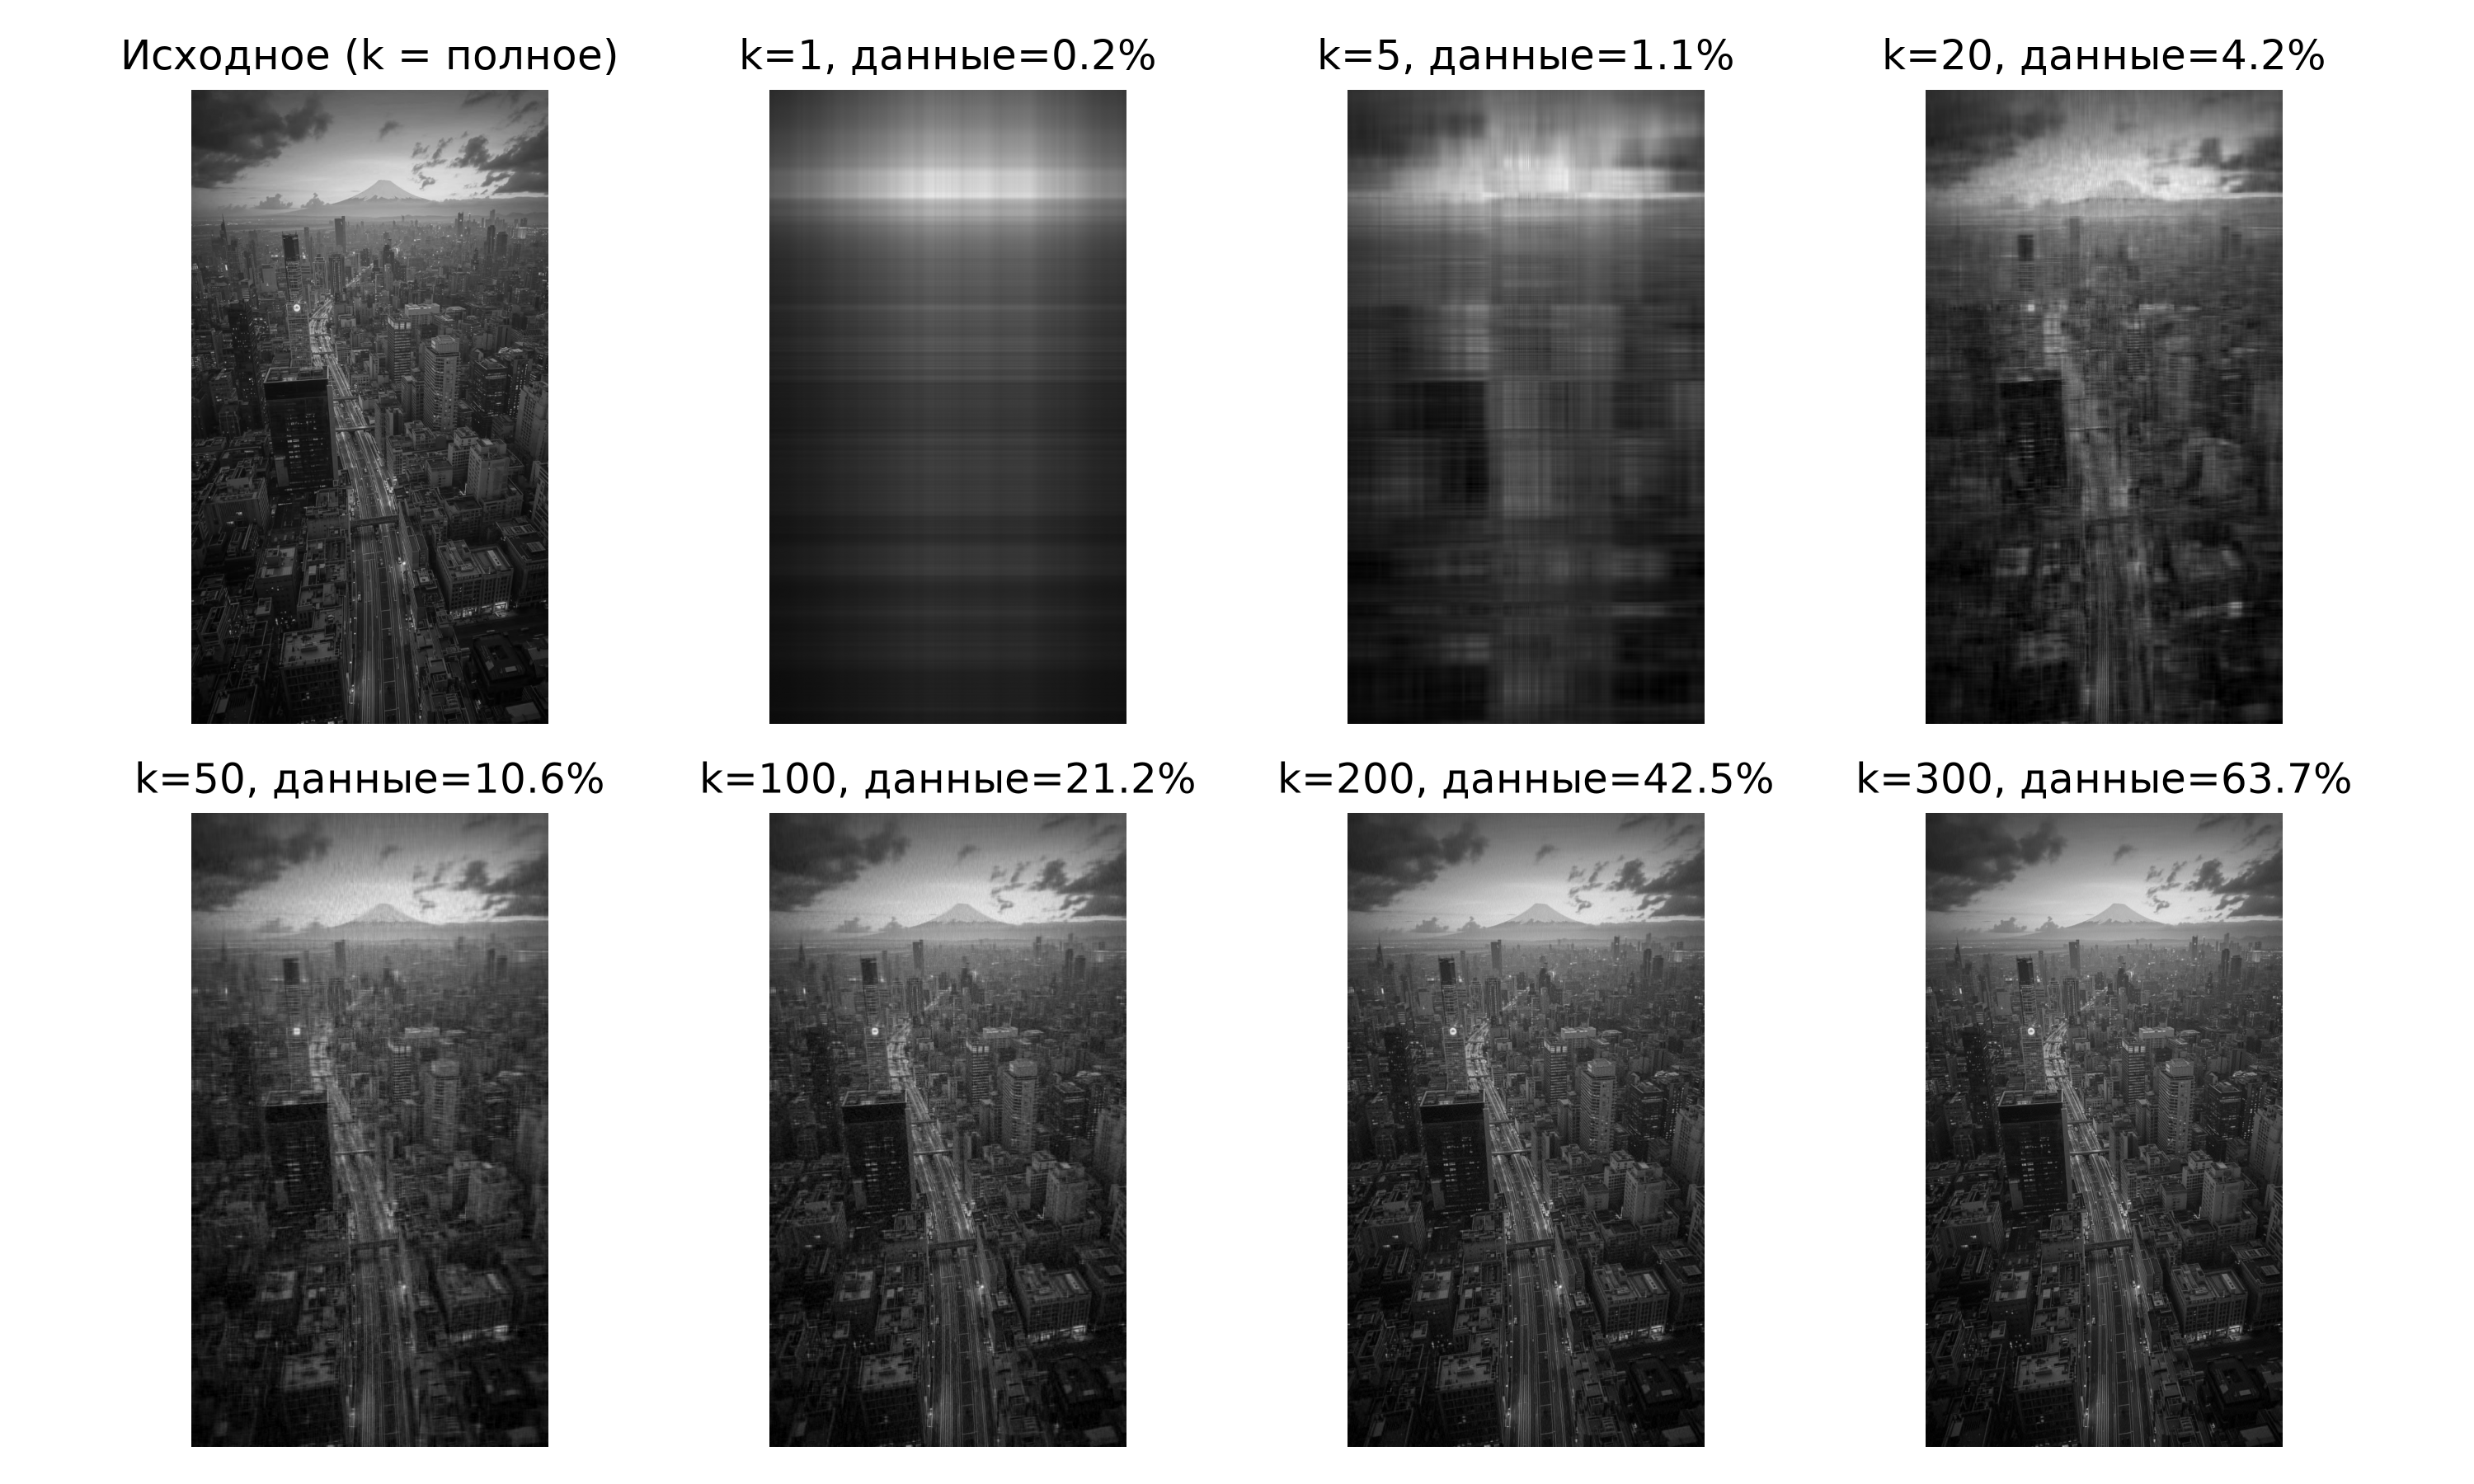
\includegraphics[width=\textwidth]{../graphics/svd_reconstructions.png}
\caption{Исходное изображение и усечённые SVD-реконструкции при различных $k$.}
\label{fig:recon}
\end{figure}

\begin{figure}[H]
\centering
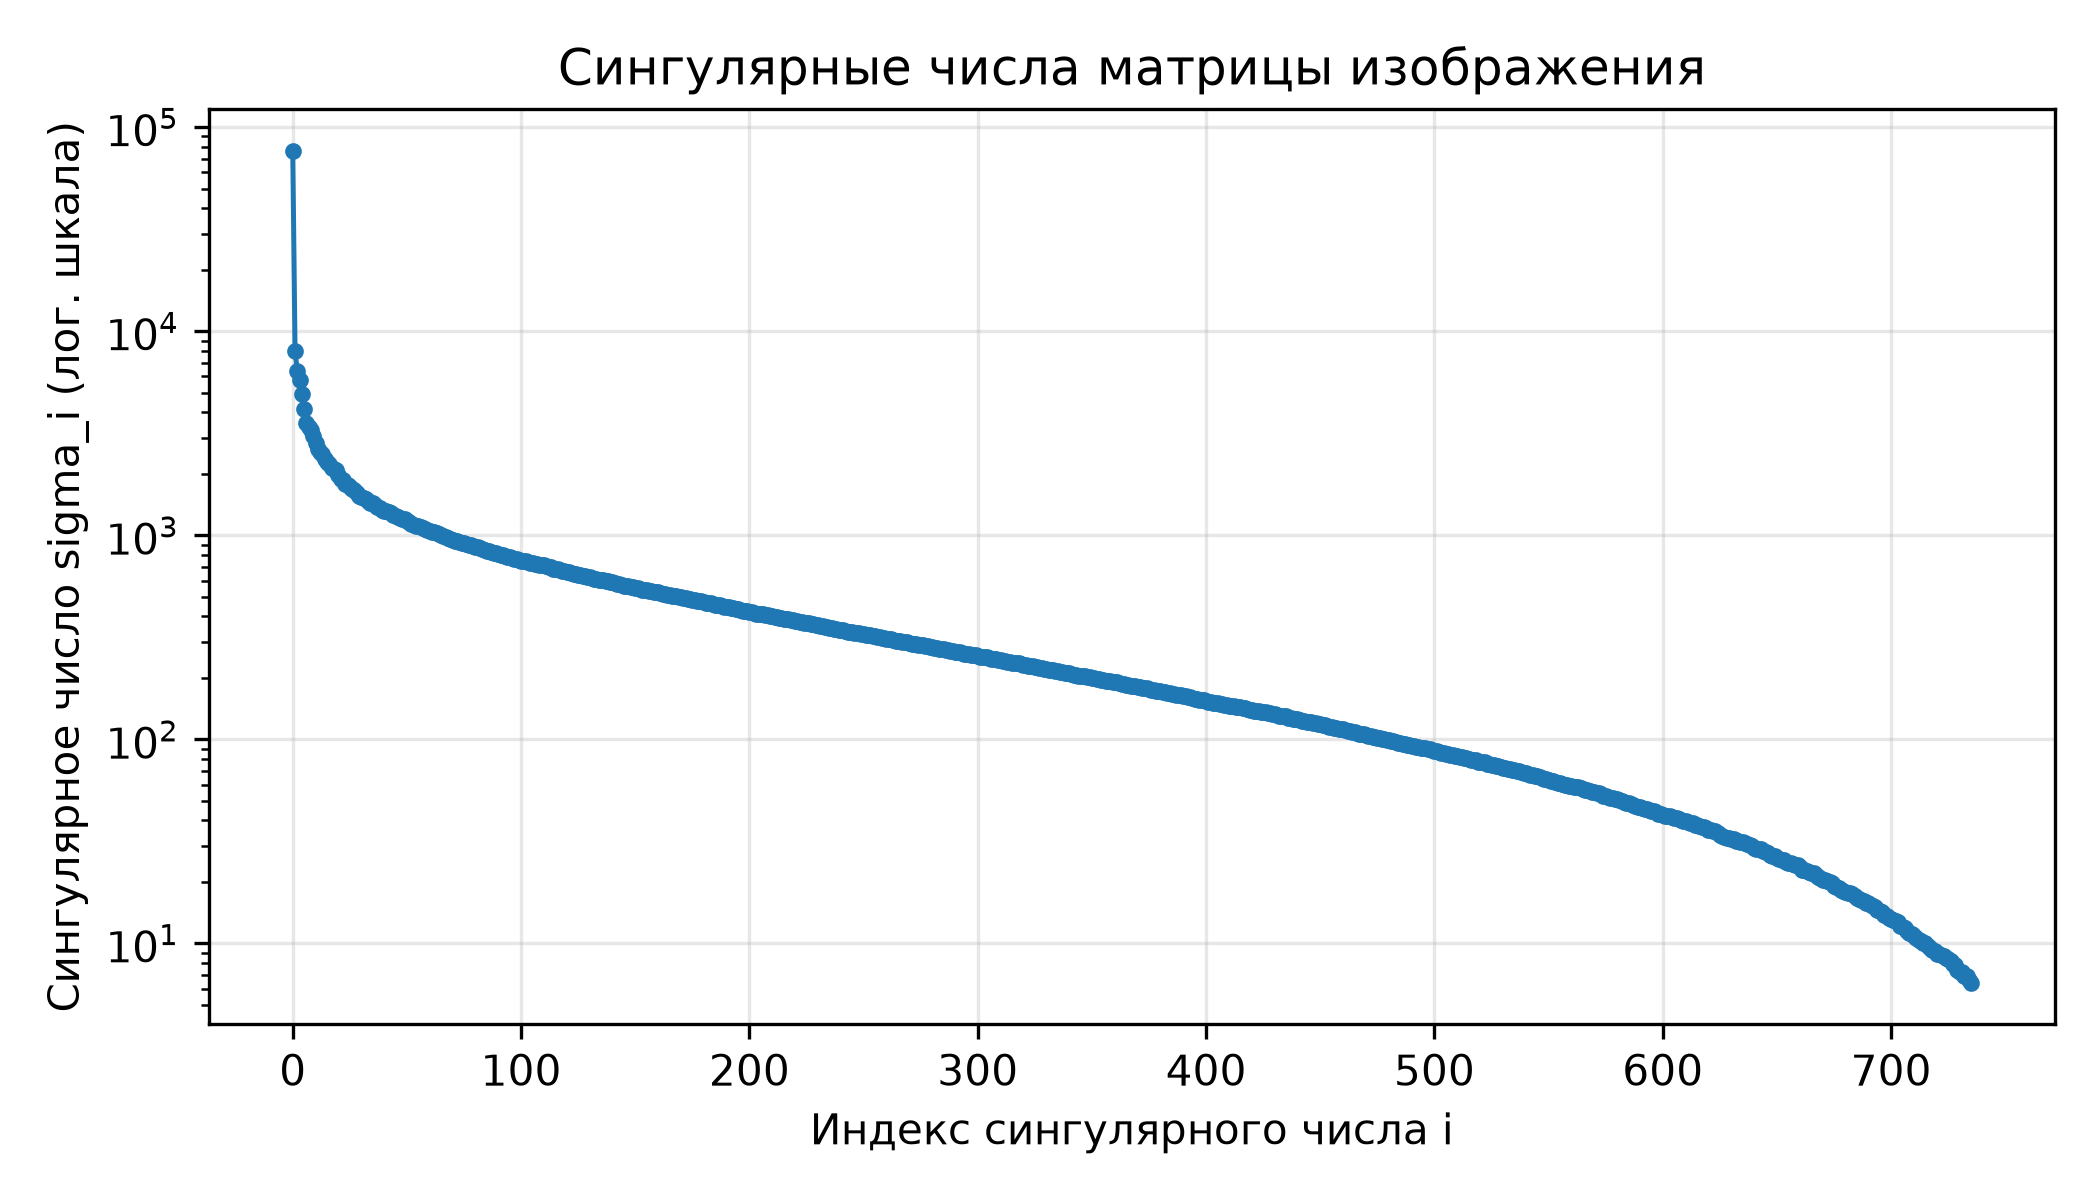
\includegraphics[width=0.95\textwidth]{../graphics/svd_singular_values.png}
\caption{Сингулярные числа матрицы изображения (лог. шкала).}
\label{fig:sv}
\end{figure}

\begin{figure}[H]
\centering
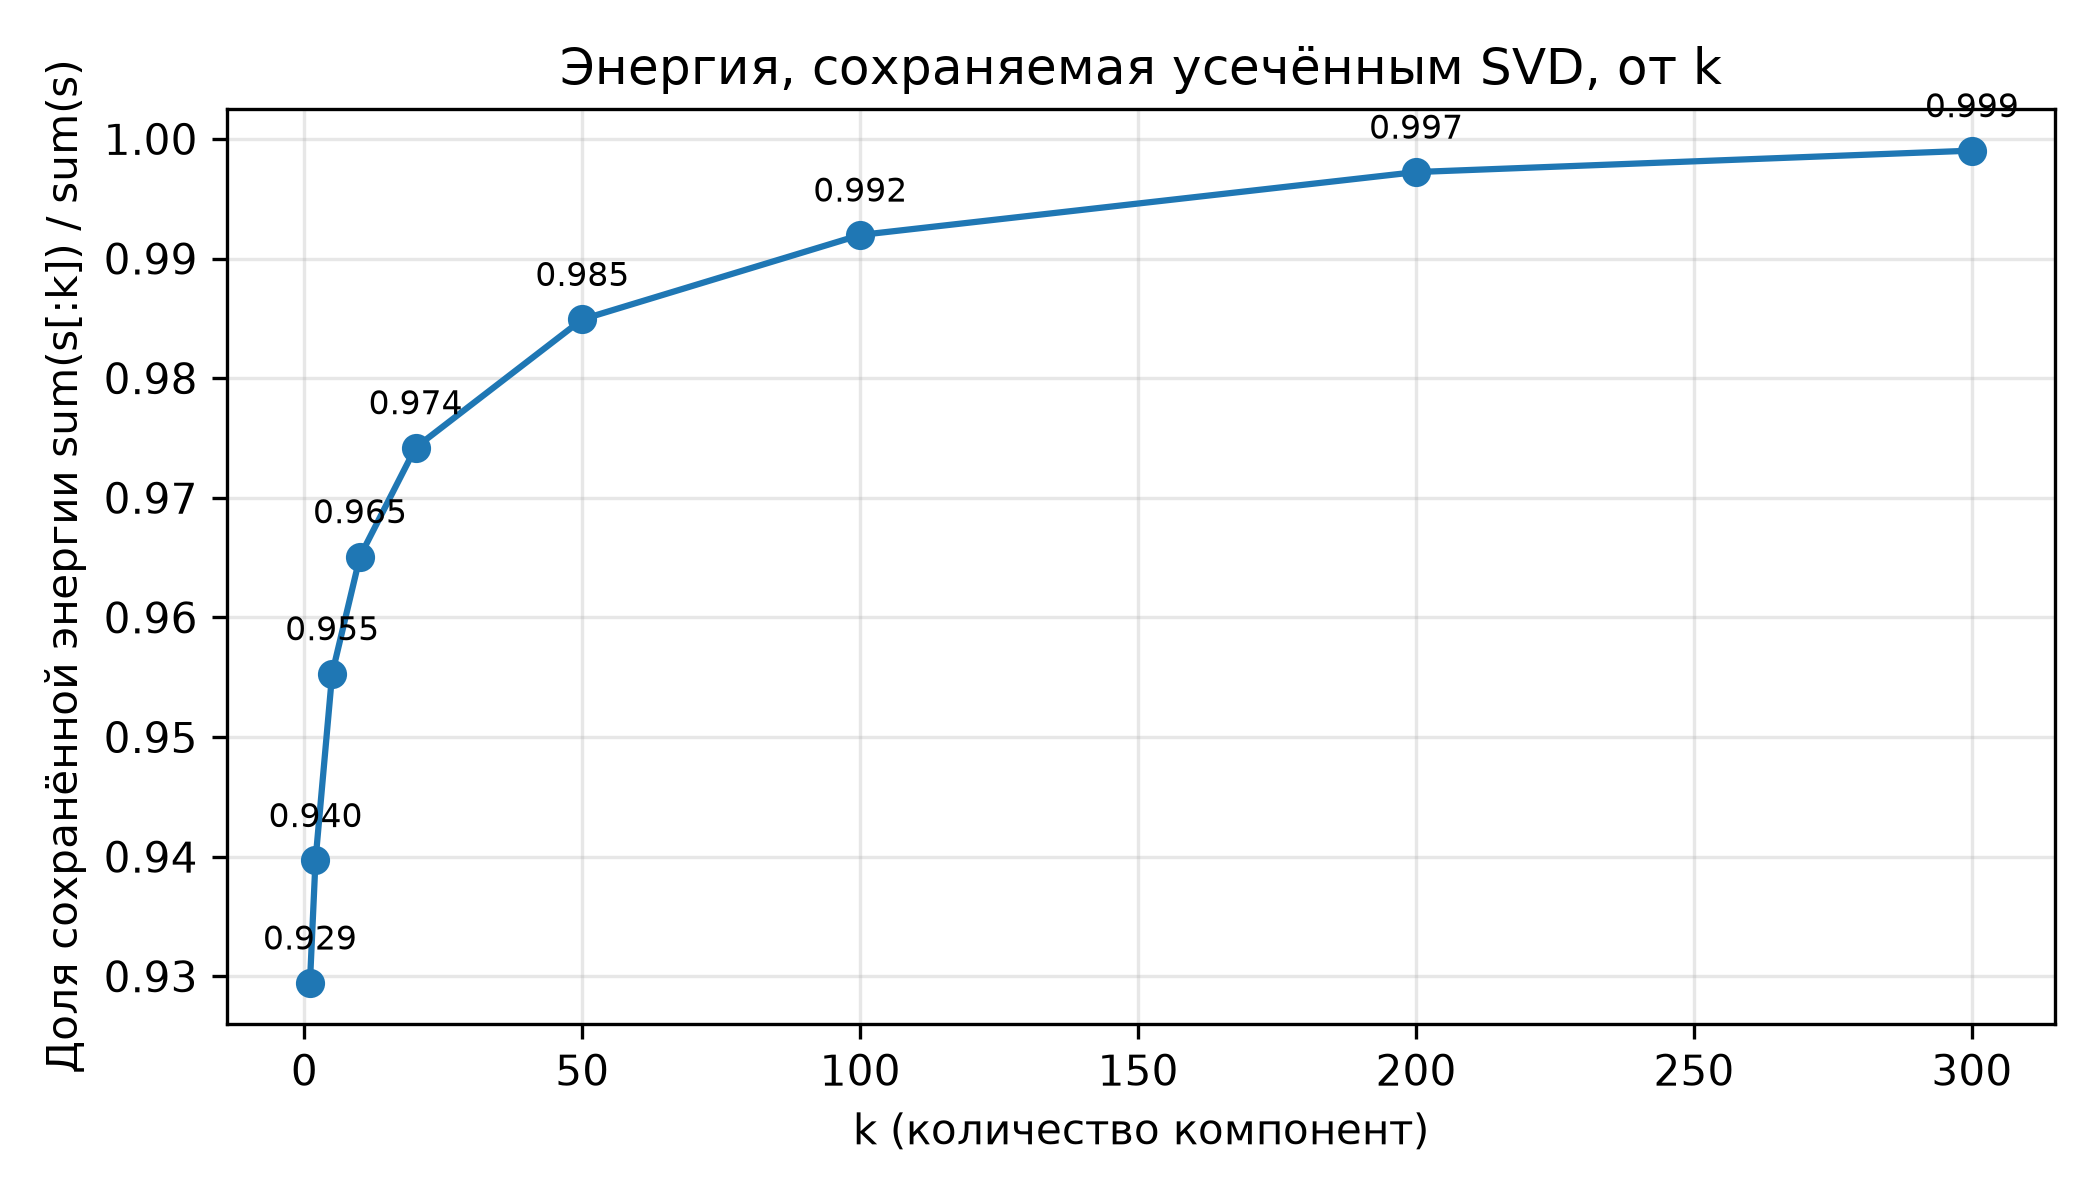
\includegraphics[width=0.95\textwidth]{../graphics/svd_energy_vs_k.png}
\caption{Доля сохранённой энергии от числа компонент $k$.}
\label{fig:energy}
\end{figure}

\begin{figure}[H]
\centering
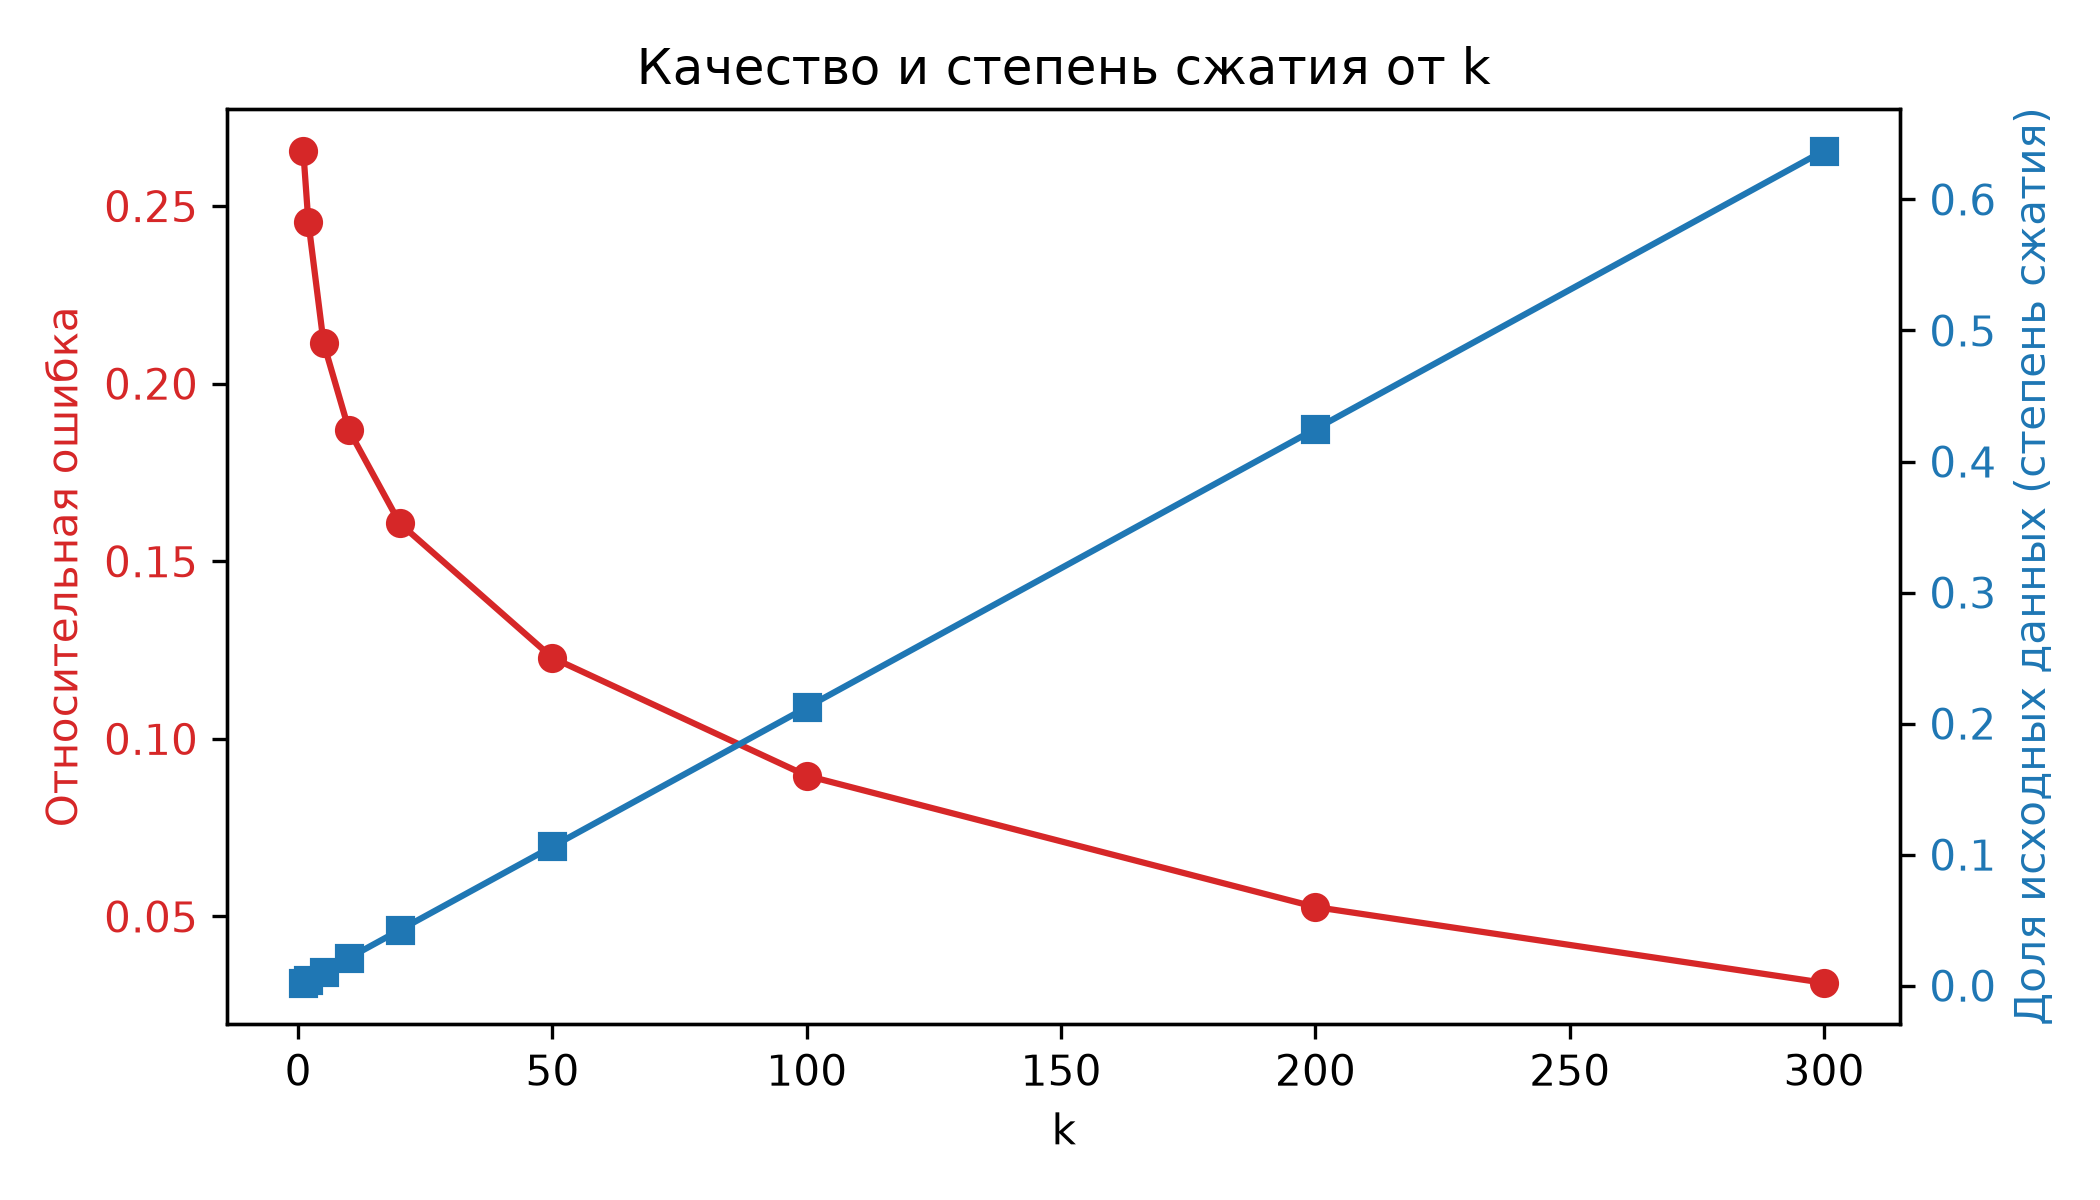
\includegraphics[width=0.95\textwidth]{../graphics/svd_quality_compression_vs_k.png}
\caption{Относительная ошибка и степень сжатия от $k$.}
\label{fig:qc}
\end{figure}

\subsection{Задание 2. LSA}
После предобработки получен словарь из 47 терминов; терм-документная матрица $A$
размера $47\times 8$. Первые два сингулярных числа:\newline
$\sigma_1\approx 3.3166$, $\sigma_2\approx 3.0409$ (доля энергии соответственно
$\approx19.0\%$ и $\approx34.9\%$ накопленного).

\begin{table}[H]
\centering
\small
\caption{Две латентные темы LSA.}
\label{tab:themes}
\begin{tabular}{c>{\raggedright\arraybackslash}p{2.2cm}>{\raggedright\arraybackslash}p{4.6cm}>{\raggedright\arraybackslash}p{3.2cm}}
\toprule
тема & сингулярное число & топ-5 слов (левый вектор) & соответствующие документы \\
\midrule
1 & 3.3166 & язык, разработка, программа, питон, программирования & Док 2, Док 1, Док 3 \\
2 & 3.0409 & хоккей, матч, команда, стадионе, сыграла & Док 6, Док 5, Док 4 \\
\bottomrule
\end{tabular}
\end{table}

Тема 1 — программирование (языки, разработка, программы), документы 1--3 подтверждают
догадку. Тема 2 — хоккей/командные виды спорта (хоккей, матч, команда, стадион),
документы 4--6 подтверждают. Документы 7--8 (кулинарные) не вошли в топ по любой из тем,
что согласуется с их содержанием.

Смысл матриц: столбцы $U$ — латентные темы в термин-пространстве; столбцы $V$ —
распределение документов по темам; сингулярные числа — значимость тем.

\begin{figure}[H]
\centering
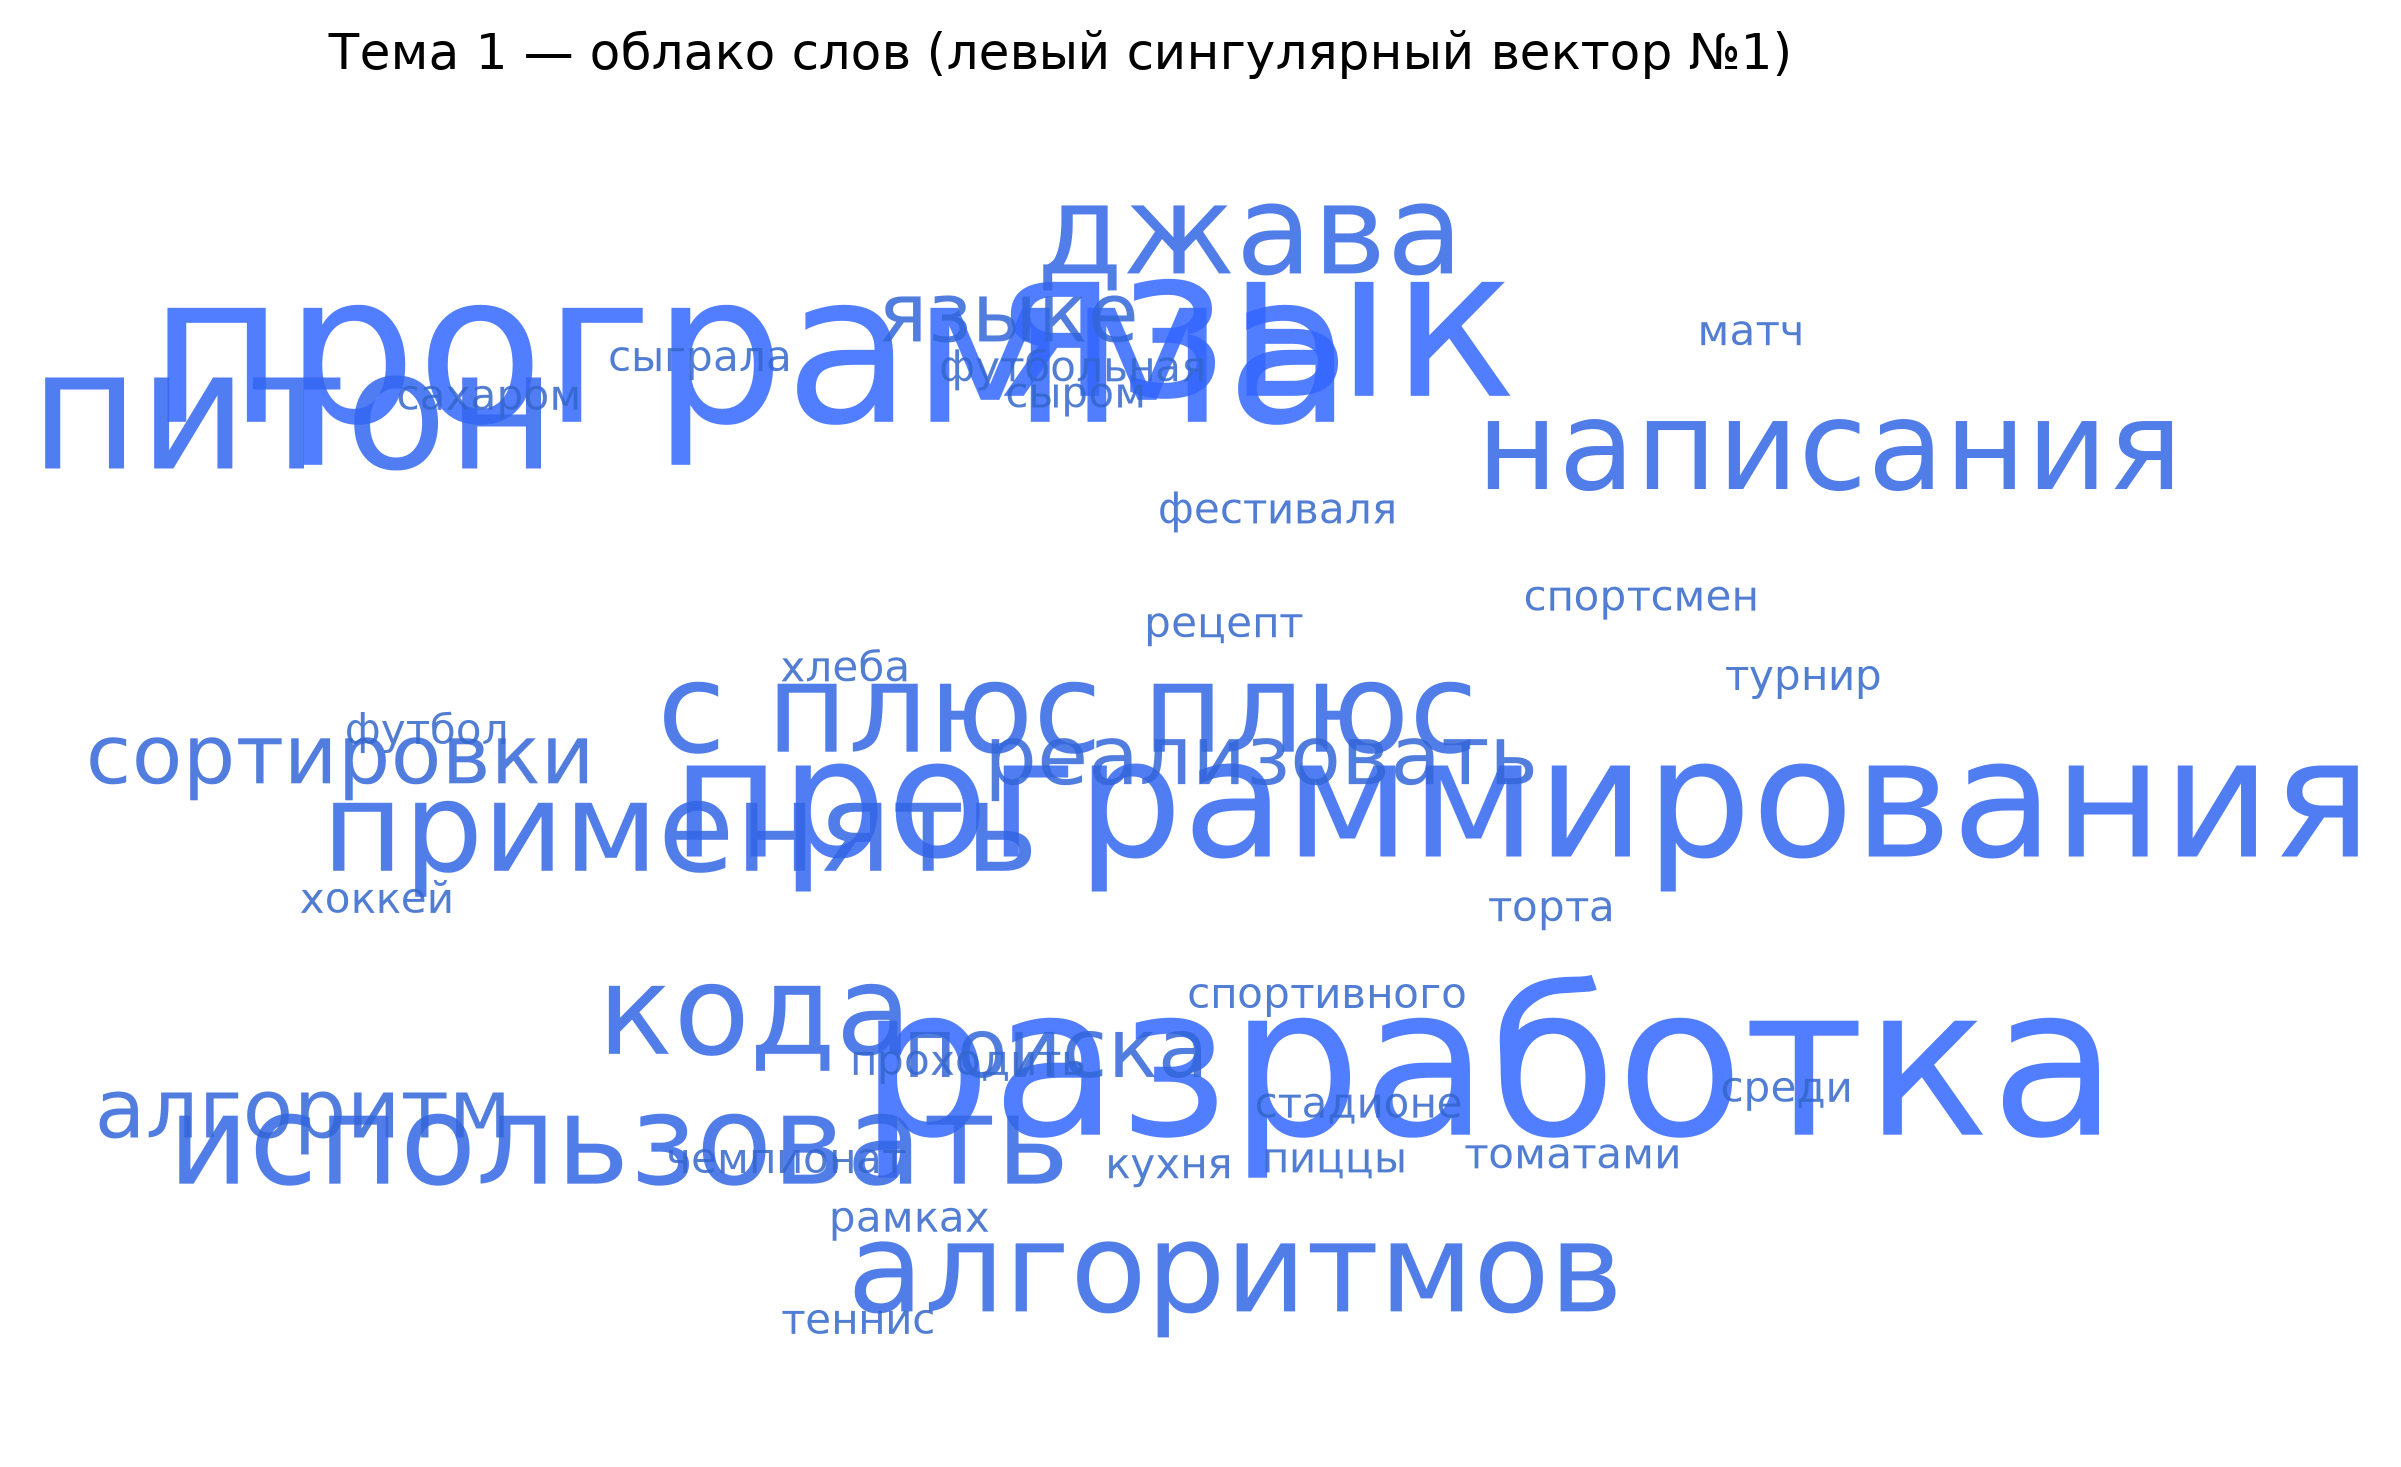
\includegraphics[width=0.47\textwidth]{../graphics/lsa_wordcloud_theme1.png}
\hfill
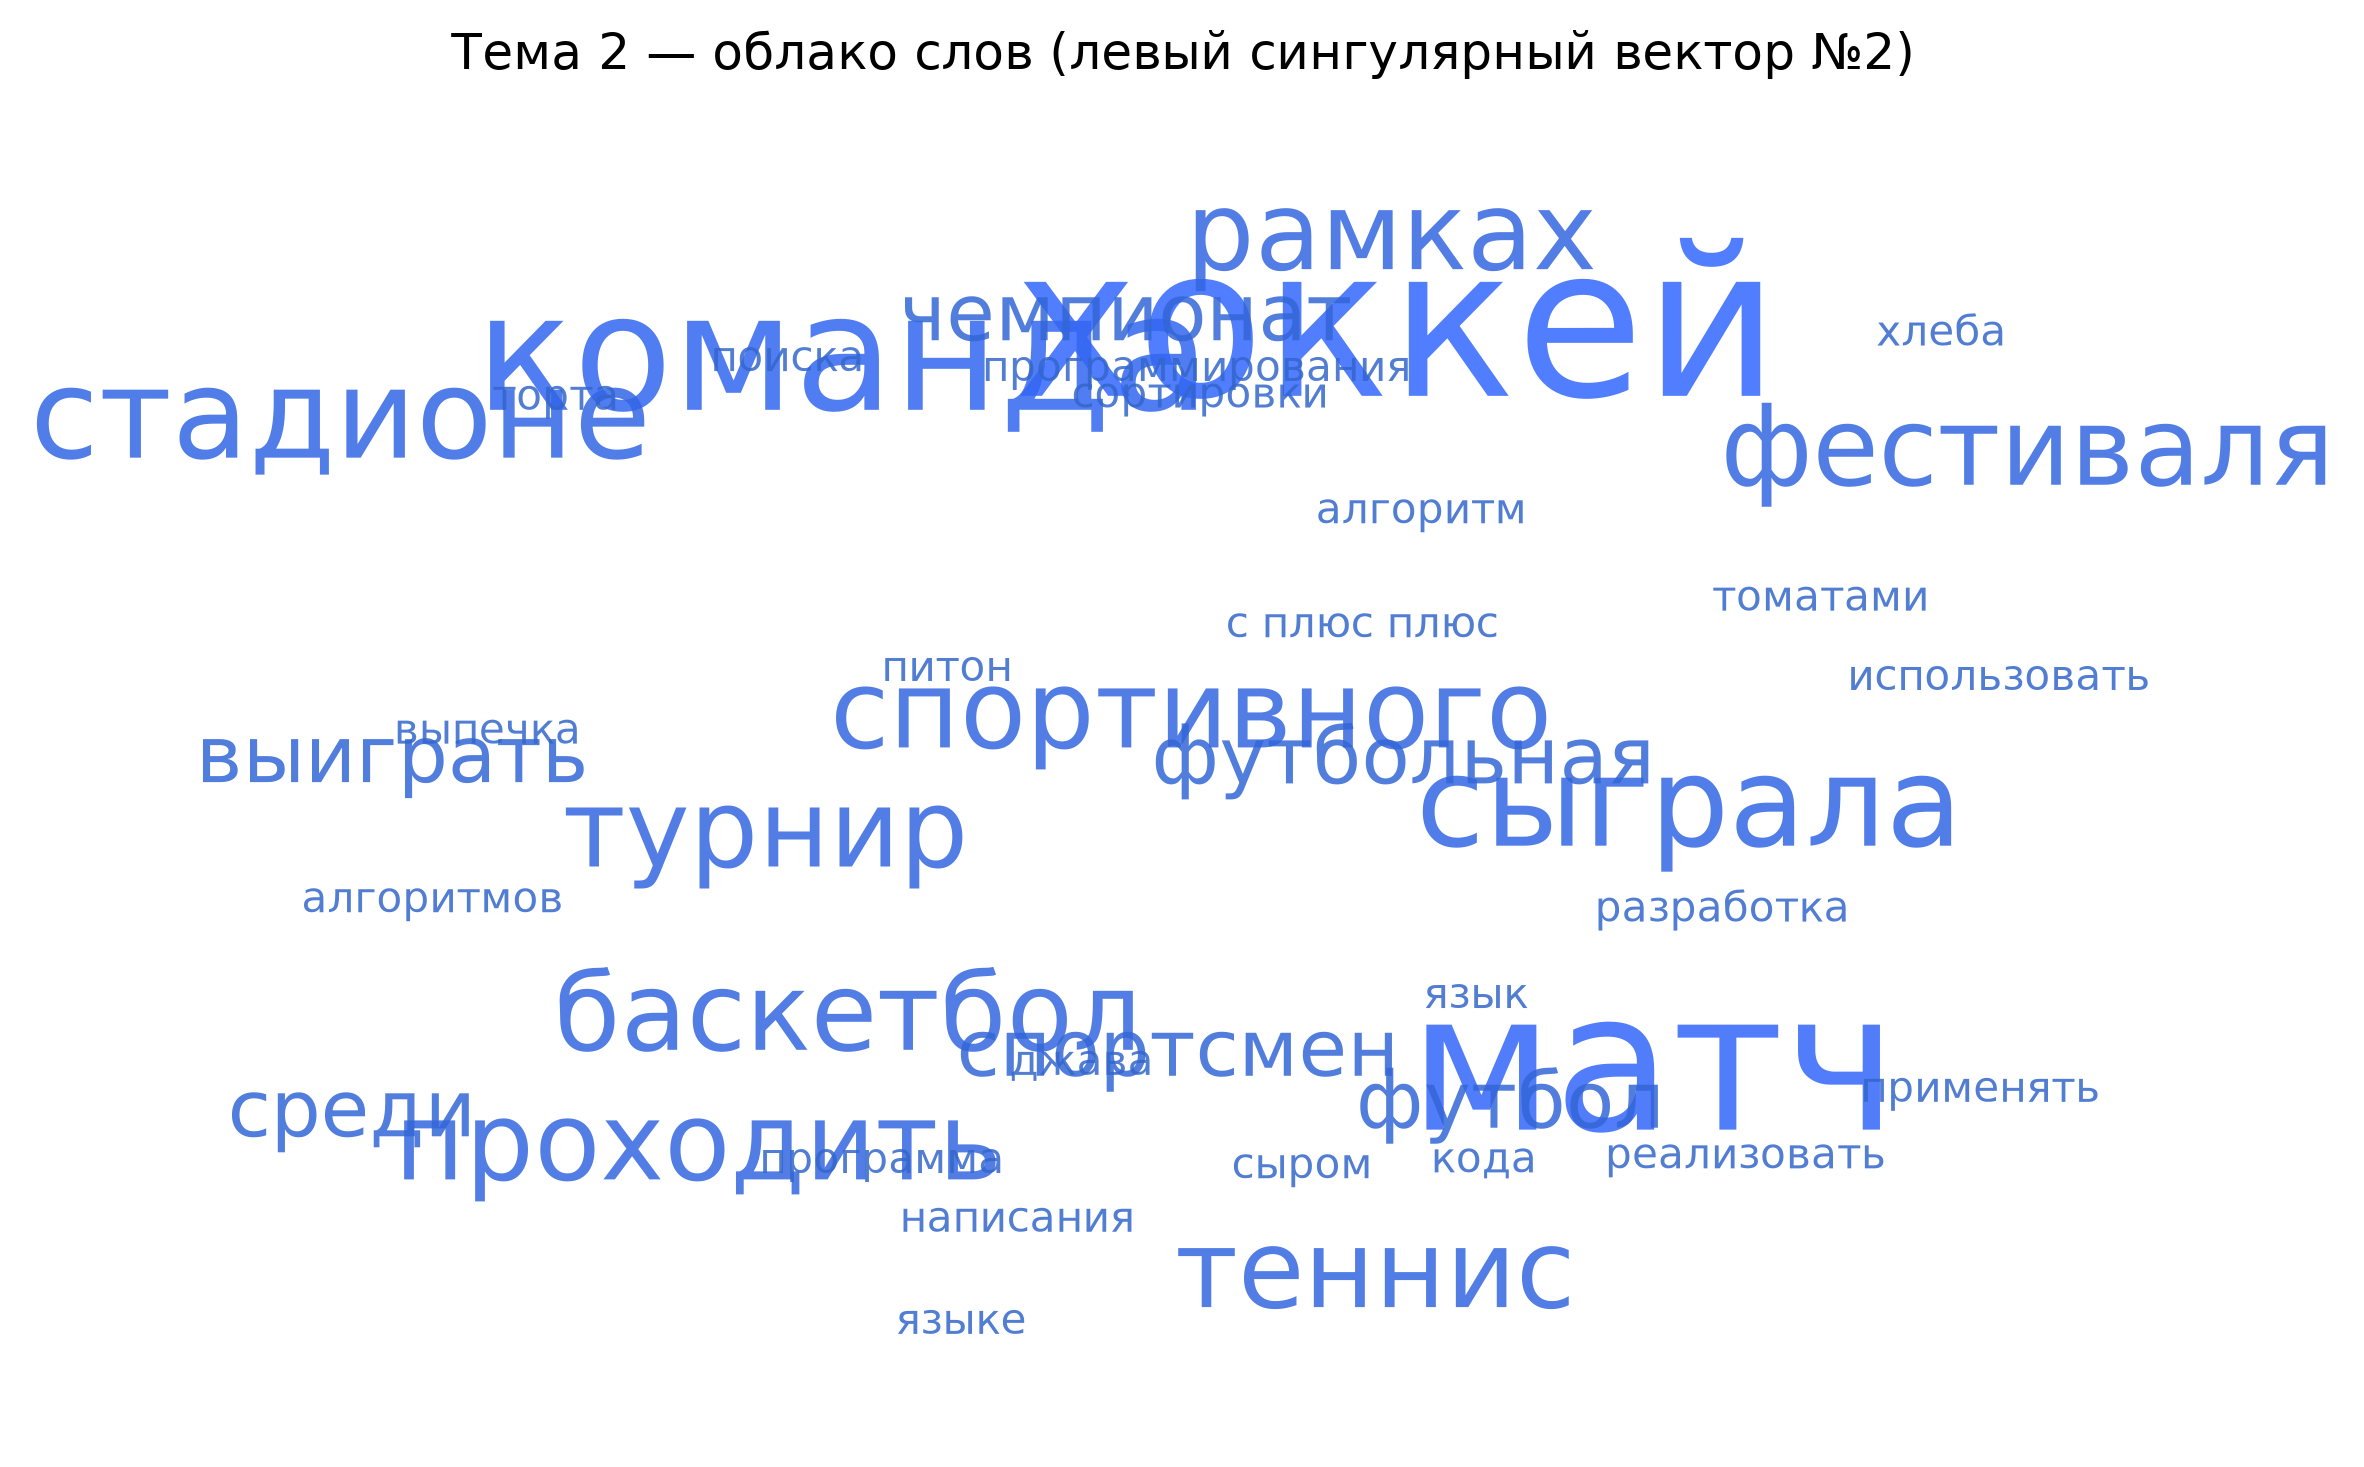
\includegraphics[width=0.47\textwidth]{../graphics/lsa_wordcloud_theme2.png}
\caption{Два облака слов по темам LSA.}
\label{fig:clouds}
\end{figure}

\begin{figure}[H]
\centering
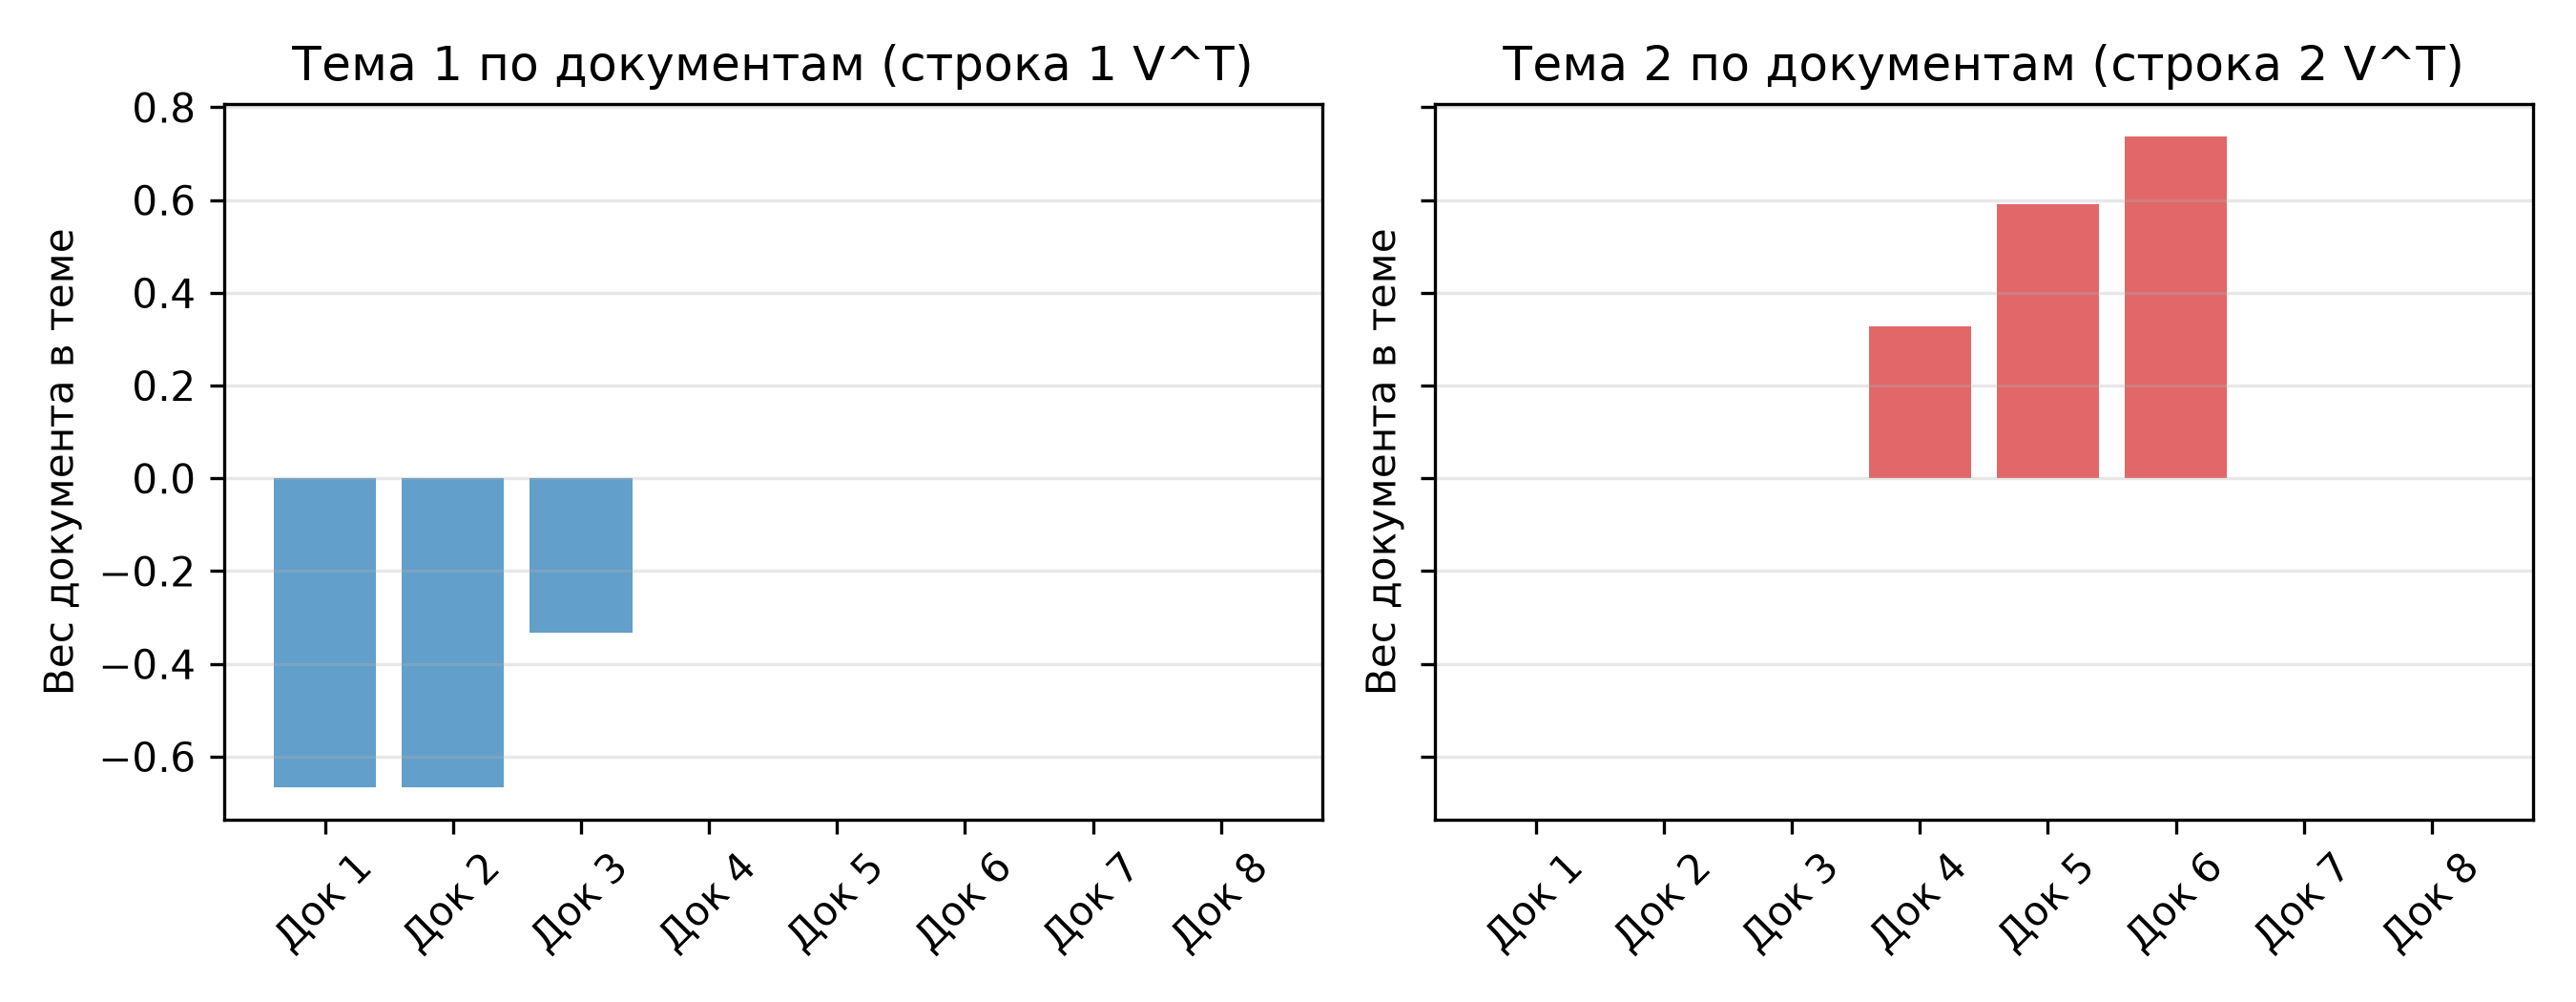
\includegraphics[width=0.95\textwidth]{../graphics/lsa_document_topics.png}
\caption{Соответствие документов темам (строки $V^\top$).}
\label{fig:docs}
\end{figure}

\begin{figure}[H]
\centering
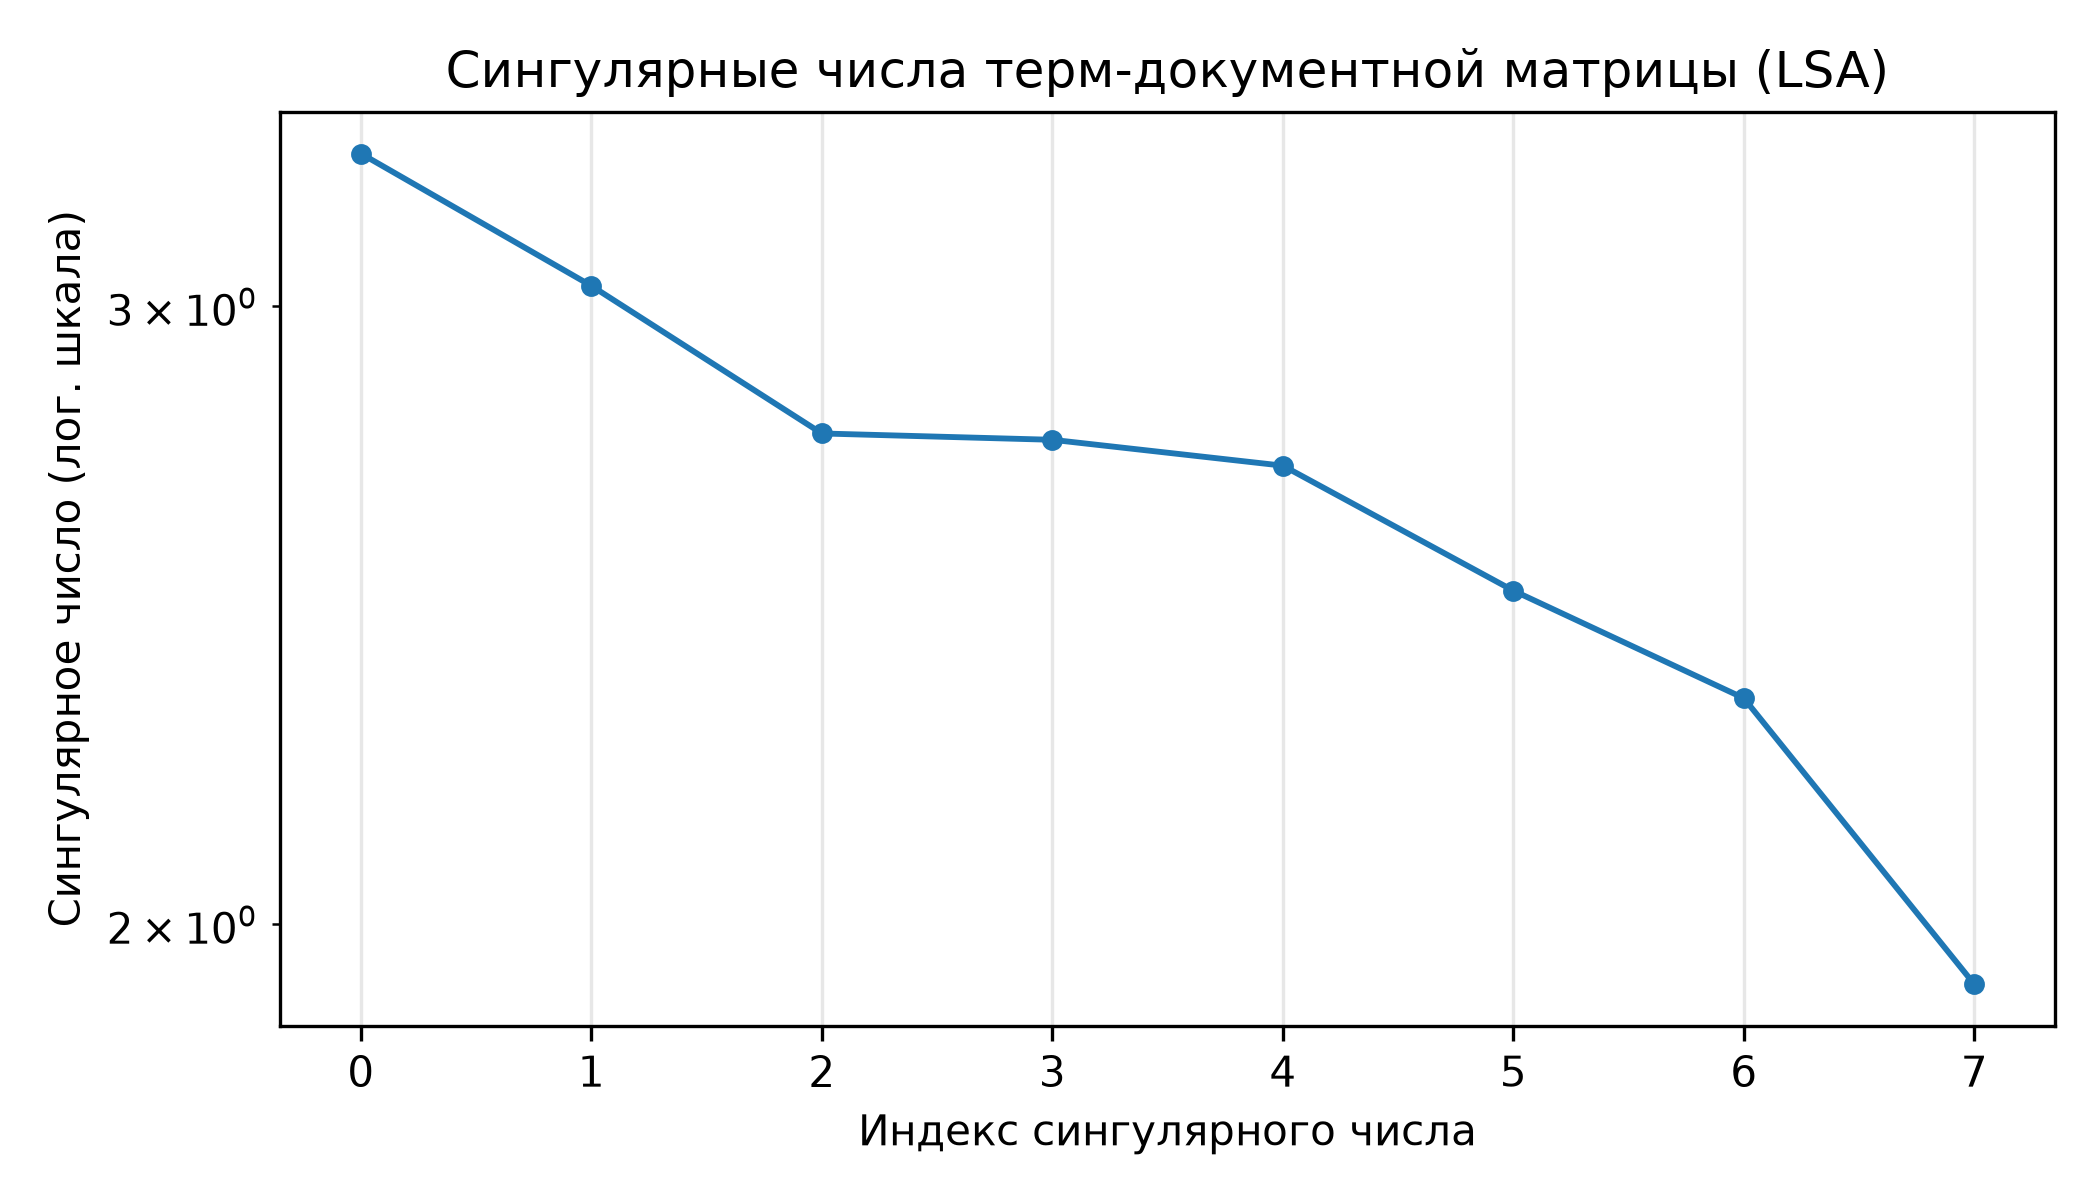
\includegraphics[width=0.95\textwidth]{../graphics/lsa_singular_values.png}
\caption{Сингулярные числа терм-документной матрицы.}
\label{fig:lsa_sv}
\end{figure}

\section{Выводы}
\begin{itemize}
    \item Сингулярное разложение даёт оптимальное по Эккарту — Янгу приближение матрицы
    низким рангом; усечённое SVD позволяет сжимать изображения: при $k=20$ сохраняется
    приемлемое качество при хранении лишь 4.25\% исходных данных, а при $k\ge100$ изображение
    почти неотличимо от исходной. При $k>470$ сжатие уже не происходит ($\gamma>1$);
    все рассмотренные $k\le300$ дают реальное сжатие.
    \item LSA на базе SVD выделяет латентные темы текстовой коллекции: столбцы $U$
    описывают темы через слова, столбцы $V$ — документы через темы, сингулярные числа —
    значимость тем. В corpora чётко разделены тема программирования и спортивная тема.
    \item Геометрический смысл SVD: поворот — масштабирование по сингулярным числам —
    поворот; сингулярные числа показывают растяжение пространства, их нулевые значения
    задают ядро, а ненулевые — образ.
\end{itemize}

\section{Приложение. Основные фрагменты кода}
\label{app:code}

Ниже приведены только минимальные фрагменты, необходимые для объяснения метода.
Полные программы сохранены отдельно.

\lstset{basicstyle=\ttfamily\tiny}

\subsection{Задание 1. Сжатие изображения (SVD)}
\label{app:svd_code}

\begin{lstlisting}[language=Python, caption={SVD-сжатие: основные фрагменты}]
import numpy as np
from PIL import Image
A = np.asarray(Image.open("source_image.jpg").convert("L"), dtype=np.float64)
m, n = A.shape
U, s, Vt = np.linalg.svd(A, full_matrices=False)
for k in [1, 2, 5, 10, 20, 50, 100, 200, 300]:
    Ak = U[:, :k] @ np.diag(s[:k]) @ Vt[:k, :]
    err = np.linalg.norm(A - Ak, "fro") / np.linalg.norm(A, "fro")
    energy = np.sum(s[:k] ** 2) / np.sum(s ** 2)
    ratio = k * (m + n + 1) / (m * n)
    print(f"k={k:3d} comp={ratio*100:.1f}% rel_err={err:.4f} energy={energy:.4f}")
\end{lstlisting}

\subsection{Задание 2. LSA}
\label{app:lsa_code}

\begin{lstlisting}[language=Python, caption={LSA: основные фрагменты}]
import re
import numpy as np
def preprocess(text):
    text = text.lower()
    text = re.sub(r"[^\w\s]", " ", text)
    tokens = [t for t in text.split() if len(t) >= 2]
    return [t for t in tokens if t not in STOP_WORDS]
doc_tokens = [preprocess(d) for d in raw_docs]
vocab = sorted({t for doc in doc_tokens for t in doc})
M = np.zeros((len(vocab), len(doc_tokens)))
for j, doc in enumerate(doc_tokens):
    for t in doc:
        M[vocab.index(t), j] += 1.0
U, s, Vt = np.linalg.svd(M, full_matrices=False)
for comp in (1, 2):
    u = U[:, comp - 1]
    top_idx = np.argsort(np.abs(u))[::-1][:5]
    top_words = [(vocab[i], u[i]) for i in top_idx]
    v = Vt[comp - 1, :]
    top_docs_idx = np.argsort(np.abs(v))[::-1][:3]
    top_docs = [(d + 1, v[d]) for d in top_docs_idx]
\end{lstlisting}

\end{document}
